\section{EKLER}
\centering\subsection{Datasheet}
    Datasheet (Veri sayfası); bilgisayar, bilgisayar bileşeni veya yazılım programı gibi bir ürün hakkında ayrıntılar sağlayan basılı veya elektronik bir belgedir. Sistemdeki elektronik elemanların datasheetleri aşağıda verilmiştir:
    
\begin{figure}[H]
\centering
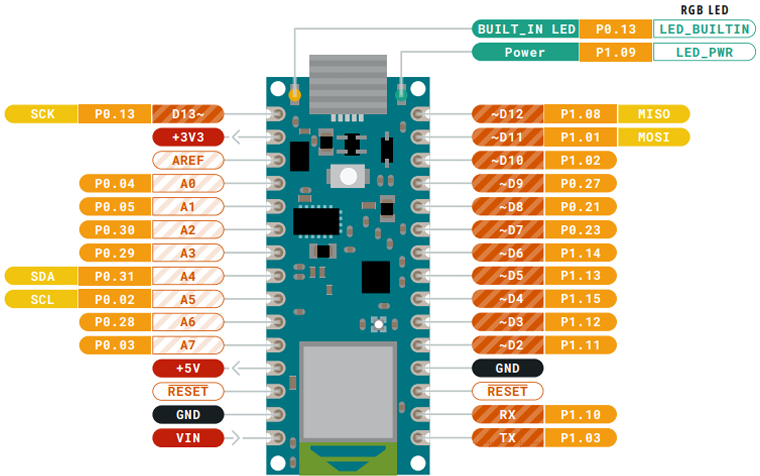
\includegraphics[width=0.55\textwidth]{Resimler/11.png}
\caption{Arduino Uno Datasheet}
\label{fig:11}
\end{figure}

\begin{figure}[H]
\centering
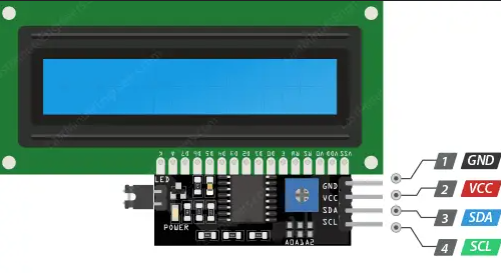
\includegraphics[width=0.55\textwidth]{Resimler/19.png}
\caption{LCD Datasheet}
\label{fig:19}
\end{figure}

\begin{figure}[H]
\centering
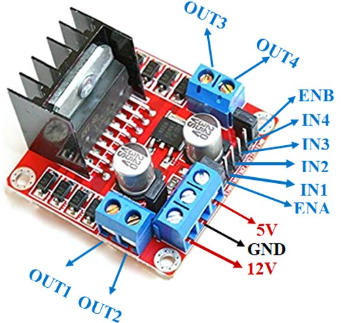
\includegraphics[width=0.55\textwidth]{Resimler/13.png}
\caption{L298N Motor Sürücü Kartı Datasheet}
\label{fig:13}
\end{figure}

\begin{figure}[H]
\centering
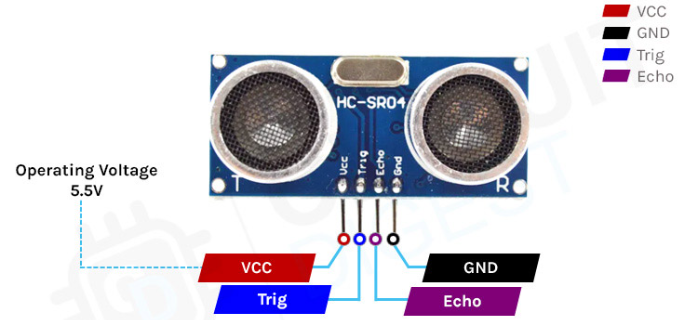
\includegraphics[width=0.55\textwidth]{Resimler/18.png}
\caption{HC-SR04 Sensörü Datasheet}
\label{fig:18}
\end{figure}

\begin{figure}[H]
\centering
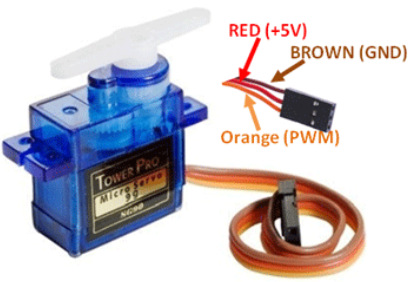
\includegraphics[width=0.55\textwidth]{Resimler/21.png}
\caption{Servo Motor Datasheet}
\label{fig:21}
\end{figure}
